\chapter{EMBASAMENTO TEÓRICO}
\label{chp:capitulo3}


SQL injections, Machine Learning utilizado, WAFs, Fuzzing e Algoritmo genetico.

\section{SQL Injection}
Discutir, resumir ponto de partida para assunto na indústria - OWASP top 10.
Artigo respectivo: An OWASP Top Ten Driven Survey on Web
https://owasp.org/www-project-top-ten/

No contexto de segurança das aplicações estudadas, Injeções de código são uma espécie de ataque ocorre quando um atacante testa a segurança de um site enviando dados inesperados para uma aplicação web, fazendo com que a mesma os processe de maneira inválida e se comporte de uma maneira diferente da qual foi originalmente programada. 

O tipo mais comum e mais prevalescente de code injection é o de SQL injection, que manipula bancos de dados via SQL (Structured Query Language), a linguagem clássica de manuseio de bancos de dados, para receber acesso a informações sensíveis.

Exemplificando algumas situações de SQL Injections:

\begin{alineas}
    \item 
    Consideremos uma aplicação que possui uma funcionalidade básica de login, com usuário e senha. Quando o usuário fornece as entradas ‘usuário’ e 123’ como credenciais, a seguinte query SQL é realizada pelo sistema na checagem:
    
    \begin{verbatim}
        SELECT * FROM users 
        WHERE username = ‘usuario’ AND password = ‘123’
    \end{verbatim}
    
    Como a query retorna os detalhes do usuário, o login é bem sucedido. Caso contrário  é rejeitado. Nesse caso, se o atacante usa a sequência de comentário SQL \textbf{--}, ele é capaz de remover a checagem de senha da cláusula \textbf{WHERE}. Exemplificando, se ele submete o usuário \textbf{administrator’--} e uma senha em branco a seguinte query é processada:
    
    \begin{verbatim}
        SELECT * FROM users 
        WHERE username = 'administrator'--' AND password = '' 
    \end{verbatim}
    
    Isso efetivamente retorna o usuário cujo username é administrator e loga o atacante como tal, expondo funções sensíveis da aplicação web inteira.


    
\end{alineas}

\begin{alineas}
    \item
    Em uma aplicação de e-commerce que organiza produtos em categorias diferentes, podemos ter um caso onde o usuário clica em uma categoria de ‘Presentes’, requisitando o seguinte URL do browser:
    
    \textbf{https://insecure-website.com/products?category=Presentes}
    
    Isso faz com que a aplicação realize uma query SQL para resgatar detalhes de tais produtos do banco de dados:
    
    \begin{verbatim}
        SELECT * FROM products
        WHERE category = ‘Presentes' AND released = 1 
    \end{verbatim}
    
    Tal query retorna todos os detalhes (identificado por \textbf{*}) da tabela de produtos, onde a categoria é \textbf{‘Presentes’} e a restrição \textbf{released} é 1. Essa restrição, quando observada por um atacante astuto, se revela como algo usado para esconder produtos não lançados. Esse atacante pode então construir um ataque digitando a seguinte URL, dado que o site não previne contra ataques SQL:
        
    \textbf{https://insecure-website.com/products?category=Presentes’--}
    
    Que provoca a seguinte query SQL:
    
    \begin{verbatim}
        SELECT * FROM products 
        WHERE category = 'Presentes'--' AND released = 1 
    \end{verbatim}
    
     Uma vez que a sequência -- anteriormente vista denota um comentário SQL, a parte depois de 
    ‘Presentes’ é interpretada como tal e não é executada, revelando todos os produtos escondidos.

\end{alineas}

\begin{alineas}
    \item
    Também é possível recuperar dados de outras tabelas de um banco de dados, utilizando a keyword \textbf{UNION}, que combina o resultado de múltiplas consultas \textbf{SELECT} em apenas um conjunto. Se um atacante executa a seguinte query contendo a entrada de usuário \textbf{`Presentes`}, ainda no último exemplo de site:
    
    \begin{verbatim}
        SELECT name, description
        FROM products WHERE category = ‘Presentes'
    \end{verbatim}
    
    Então ele pode também submeter uma entrada nociva com \textbf{UNION}:
    
    \begin{verbatim}
        ' UNION SELECT username, password FROM users--
    \end{verbatim}
        
    Tal entrada faz com que todos os usuários e senhas venham juntos das descrições dos supostos presentes, fundamentalmente comprometendo a segurança da aplicação

\end{alineas}

A prevenção de vulnerabilidades deste tipo são dependentes das tecnologias em uso na aplicação web. Porém, alguns ponteiros básicos podem ser indicados - o uso de uma API segura, que evite o uso do interpretador SQL inteiramente ou use uma interface parametrizada; validação server-side de input positiva ou com “allowlist”; uso de queries LIMIT e outras queries SQL de controle no interpretador para evitar que informações sejam divulgadas em massa. Sumariamente, separar dados da lógica da aplicação web, e implementar configurações e/ou restrições que limitem a exposição dos dados nos casos de code injections bem sucedidas. 

No contexto deste trabalho, no entanto, é estudado uma forma tanto comercial como open-source que têm tido crescimento no mercado: o uso de Web Application Firewalls, mais especificamente o de Web Application Firewalls baseados em técnicas de Machine Learning.

TO-DO: Colocar citações desse trecho de trabFinalMab.pdf 

\section{OWASP TOP 10}

Há pelo menos dez anos os ataques cibernéticos vem aumentando, tendo grande impacto nas empresas.
Aplicações web quando são desenvolvidas sem ter segurança da informação no seu cerne possibilita perda de ativos, inoperabilidade de serviços, exposição de dados sensíveis e comprometimento de sistemas. 
A Open Web Application Security Project (OWASP) é uma fundação sem fins lucrativos cujo objetivo é aprimorar a segurança do software. A organização fornece projeto de código livre, vasta comunidade ativa, conferências, treinamentos e boas práticas. Uma das iniciativas é o OWASP TOP 10, que significa as 10 vulnerabilidades mais comuns:

1) Injeção;
2) Broken Authentication;
3) Exposição de Dados Sensíveis;
4) Entidades Externas de XML;
5) Broken Access Control;
6) Configurações Incorretas de Segurança;
7) Cross Site Scripting XSS;
Design inseguro;
Componentes vulneráveis e desatualizados;
Falhas de identificação e autenticação;
Falhas de integridade de software e dados;
Falhas de monitoramento e security logging;
Server-Side Request Forgery (SSRF).

Injeção
Forma de ataque ampla onde uma entrada de dados recebe caracteres não tratados que são executados pelo sistema com objetivo de alterar o funcionamento padrão do software.
Uma das formas mais conhecidas de injeçao é o SQL Injection. Aplicações vulneráveis a SQL injection geralmente permitem a obtenção completa dos dados do banco de dados e execução de códigos arbitrários remotamente. Existem variantes do SQL Injection como: error-based, union-based, blind e out-of-band. Error-based são injeções que fornecem erros de SQL para o atacante, vazando informações críticas do banco de dados. Union-based são ataques que utilizam uma query existente na lógica do sistema concatenada a outra através de um UNION de maneira a executar uma segunda lógica além da já estabelecida pelo sistema. Injeções às cegas (blind-based) são aquelas que o sistema não dá nenhuma informação após a injeção, de forma que o atacante precisa ser engenhoso para obter informações e prosseguir com a ofensiva. Out-of-band é uma injeção sem o fornecimento de um output para o atacante, porém é possível redirecionar a saída para um endpoint, geralmente servidor http.
É fundamental para mitigar as injeções ter uma validação dos caracteres e declarações válidas ao receber uma entrada de dados na aplicação web.

Broken Authentication
Broken Authentication é um conjunto de métodos em que os atacantes podem ganhar as credenciais de usuário ou sequestrar sessões de usuário. Senhas fracas ou facilmente adivinháveis, senhas armazenadas indevidamente sem serem transformadas em hashes, IDs de sessão expostos em URLS, ataques de fixação de ID de sessão e transmissão não-criptografada http.
Para mitigar problemas dessa natureza são indicadas medidas como armazenar senhas com hash, garantir que IDs de sessão não estão expostos nas URLS, configurar timeouts nas sessões, não permitir recriação de sessões expiradas, não transmitir senhas em canais sem criptografia, utilizar senhas com tamanho mínimo e determinada complexidade, ocultar nomes de usuário e senha em mensagens de erro devido a login mal sucedido e assegurar proteção contra brute force após cinco tentativas falhas.

Exposição de Dados Sensíveis
Aplicações web que não protegem senhas, informações financeiras ou relativas servindo potencialmente para criminosos obterem acesso não autorizado a contas de usuário, efetuar ações fraudulentas como compras online com informações roubadas ou extorquir vítimas com dados sensíveis. Dados sensíveis expostos podem causar perdas financeiras, ferir a reputação de corporações que tiveram seus dados vazados ou ativos expostos, levando as empresas a pagarem despesas para investigação sobre o incidente de segurança. Para proteger-se desse tipo de ataque são necessários softwares de acordo com a legislação do país e da industria, uma vez que ignorar a possibilidade de exposição de dados sensíveis leva a desastres financeiros de grandes proporções. 

Entidades Externas de XML
Um tipo particular de injeção, também conhecido como injeção XXE, ocorre quando atacantes abusam dos parses XML utilizados em servidores web através do envio de documentos XML cuidadosamente forjados que caso sejam processados levam à negação de servição, execução remota de código arbitrário ou requisições forjadas do lado do servidor.
Por exemplo, um atacante pode enviar um payload especialmente forjado para um servidor web, o servidor web envia para um parser XML, o parser XML por sua vez devolve o caminho do arquivo para o servidor, que devolve para o agente malicioso.

\begin{verbatim}
    <?xml version="1.0" ?>
    <!DOCTYPE passws [
    <!ELEMENT passwd ANY>
    <!ENTITY passwd SYSTEM "file:///etc/passwd">
    ]>

    <passwd>&xxe;</passwd>
\end{verbatim}

Existem duas variantes de ataques XXE, sendo a primeira conhecida como in-band, onde o atacante forja um documento XML malicioso e o submete através da rede para ser processado e recebe uma resposta instantânea, enquanto a outra variante chamada out-of-band ocorre quando o atacante forja um documento XML malicioso, submete, todavia não obtém resposta imediata do servidor web. Ataques out-of-band também são chamados de "blind XXE injection".
É possível mitigar injeções XXE desativando o Document Type Definitions (DTD). 

Broken Access Control
Diversos vetores de ataque podem ser considerados Broken access control. Entre eles: burlar verificações de controle de acesso, editar contas de outros usuários, elevação de privilégios, configurações erroneas de CORS (Cross-Origin Resource Sharing) que permitem acesso não autorizado a APIs (Application Programming Interface) restritas, manipulação de metadados através de tokens de controle de acesso JWT (JSON Web Tokens) e acesso não autorizado a páginas web com usuário desprivilegiado, podendo levar ao controle de funções do modelo de negócio ou obtenção de (todos) os dados.
É recomendado ter listas de controle de acesso e negar funcionalidades através de back-end, de forma que o usuário não tem acesso ou controle do código.

Configurações Incorretas de Segurança (Security misconfigurations)
Configurações errôneas de segurança podem expor aplicações a security threads. Portas administrativas abertas desnecessariamente, firewalls mal gerenciados, aplicações legadas tentando comunicar com outras aplicações inexistentes são alguns exemplos de possíveis ingerencias nas configurações de segurança. São necessários padrões de qualidade, revistos, testados e verificados com frequencia para reduzir a superficie de ataque que esse tipo de vulnerabilidade permite.

Cross Site Scripting XSS

Referências:

Understanding The Top 10 OWASP Vulnerabilities, Matthew Bach-Nutman

https://arxiv.org/ftp/arxiv/papers/2012/2012.09960.pdf

https://www.indusface.com/blog/10-common-web-application-security-mistakes/

https://www.invicti.com/learn/out-of-band-sql-injection-oob-sqli/

https://owasp.org/www-project-top-ten/

shorturl.at/ewHNS

https://www.acunetix.com/blog/web-security-zone/what-is-session-fixation/

TODO:
botar imagem com as top 10 vulnerabilidades
arrumar as referências
verificar acentuação
melhorar listagem de acordo com padrão tcc
verificar se vale a pena deixar alguns termos em ingles tipo broken access control
Organizar subtitulos
No final relacionar injeção com nosso trabalho
Verificar se entrou/saiu algo do owasp moderno
trocar os 2 blogs por livros ou artigos



\section{Algoritmo Genético}

Explicar mutation rounds, funcionamento de pool e como fuzzer se encaixaria

\section{Algoritmos de Fuzzing}

O cerne do algoritmo por trás do WAF-A-MoLE e o WAF-A-MoLE++ se encontra na técnica de \textit{fuzzing}. O termo fuzz foi cunhado pelo professor da Universidade de Wisconsin-Madison Barton Miller nos anos 80, após sofrer uma interferência considerável de uma tempestade no funcionamento de aplicações que rodavam em um ambiente unix remoto na época. 

Pouco depois disso o mesmo passou aos seus alunos uma tarefa denominada o \textit{"Fuzz Generator"}, na qual era necessário implementar uma ferramenta que testasse a robustez de programas unix através de um bombardeio de informações aleatoriamente geradas.

Atualmente é uma técnica amplamente aceita na testagem/sondagem da segurança de diversas aplicações, com um leque de ofertas de fuzzing comerciais no mercado. E naturalmente é empregável em Web Application Firewalls, permitindo extrair informações valiosas que rendam aprimoramentos para os mesmos.

Uma função elementar de fuzzing, pode ser vista abaixo:

\includecode[C]{Função de um fuzzer elementar} {alg:codigo1}{codigos/fuzzer.py}

\bigskip
Tais funções de fuzzing podem ser aprimoradas, customizadas para testar os mais diversos programas. Uma das maneiras de polir os resultados oriundos de fuzzing elementar, que podem ser rejeitados facilmente por muitos programas inicialmente, é um processo chamado fuzzing mutacional, ou \textit{mutational fuzzing}, projetado para melhorar as chances de obter entradas consideradas válidas.

Nessa estratégia, a execução se inicia com uma entrada válida, e ela subsequentemente sofre uma mutação pequena, como no caso de uma string a mudança de um caractere, adição/remoção de um número, ou até mesmo uma troca de um bit (todos naturalmente aleatórios, pelo princípio do funcionamento de fuzzing).

\includecode[C]{Classe de fuzzer mutacional} {alg:codigo1}{codigos/mutational_fuzzer.py}

\bigskip
O programa acima realiza, dentre 3 operadores de mutação, uma mutação aleatória ao chamar a função mutate(). Na prática, são realizadas uma série de mutações para que se produzam entradas viáveis. Com um simples loop para chamar mutate isso é possibilitado.

O contexto relevante para o WAF-A-MoLE é produzir, iterativamente juntamente com o Algoritmo Genético anteriormente descrito, múltiplas injeções SQL a serem testadas a cada "rodada" de mutação. Uma injeção SQL é usada como base inicial, e a mesma sofre mutações por um fuzzer dedicado até ser considerada válida pelo Web Application Firewall testado, embora seja no fundo ainda uma injeção maliciosa.


Resumidamente, o WAF-A-MoLE++ pode ser descrito como um fuzzer genético, operando em cima de WAFs com entradas "fuzzeadas".

Referências:
https://www.fuzzingbook.org/html/Fuzzer.html
https://www.fuzzingbook.org/html/MutationFuzzer.html
https://fuzzinginfo.wordpress.com/history/

\section{Recurrent Neural Networks}

Para cada um desses, explicar o algoritmo com o funcionamento base, e o funcionamento no Contexto de WAF. Explicar aonde no WAF-A-MoLE entra caso já não tenha sido mencionado. 

\section{Naive Bayes}

\section{Random Forest}

\section{Support Vector Machine}

\subsection{Linear SVM}

\subsection{Gaussian SVM}






Texto.

\subsection{Seção Terciária}

Alíneas e subalíneas.
\bigskip

\begin{alineas}
\item linha 1:
\begin{alineas}
\item subalinea 1;
\item subalinea 2;
\end{alineas}
\item linha 2:
\begin{subalineas}
\item subalinea 1;
\item subalinea 2;
\end{subalineas}
\item linha 3:
\begin{incisos}
\item subalinea 1;
\item subalinea 2;
\end{incisos}
\item linha 4.
\end{alineas}


\section{Exemplo de Tabelas, Quadros e Figuras}

{\centering\bfseries\color{red}
Exemplo de Tabela
\par}

\begin{table}[ht]
\centering
\caption{Preços de alimentos em dólares de 1900-1952 a
1995-1997}
\begin{supertabular}{m{3.6cm}m{3.7cm}m{3.6cm}m{3.0cm}}
\hline
\multicolumn{1}{m{3.636cm}|}{\centering{ ALIMENTO}} &
\multicolumn{1}{m{3.741cm}|}{\centering{ 1950-1952}} &
\multicolumn{1}{m{3.635cm}|}{\centering{ 1995-1977}} &
\centering\arraybslash{ VARIAÇÃO PERCENTUAL}\\\hline
\centering{ Trigo} &
\centering{ 427,6} &
\centering{ 159,3} &
\centering\arraybslash{ {}-62,7}\\
\centering{ Arroz} &
\centering{ 789,7} &
\centering{ 282,3} &
\centering\arraybslash{ {}-64,2}\\
\centering{ Sorgo} &
\centering{ 328,7} &
\centering{ 110,9} &
\centering\arraybslash{ {}-66,2}\\
\centering{ Milho} &
\centering{ 372,0} &
\centering{ 119,1} &
\centering\arraybslash{ {}-68,0}\\\hline
\end{supertabular}
    \legend{Fonte: Sen (2000, p. 240). }
    \label{tab:alimentos}
\end{table}

\bigskip

{\centering\bfseries\color{red}
Exemplo de Quadro
\par}

\begin{quadro}[htb]
\centering
\caption{Comparativo de competitividade}
\begin{supertabular}{|m{2.5cm}|m{2.5cm}|m{6.0cm}|m{3.2cm}|}
\hline
{ EMPRESA } &
{ PRINCIPAL MATÉRIA-PRIMA } &
{ ALTERNATIVAS DE SUPRIMENTOS PARA A PRINCIPAL MATÉRIA-PRIMA } &
{ FLEXIBILIDADE }\\\hline
{ Copesul } &
{ Nafta } &
{ Disponibilidade de produto na Argentina} &
{ 45\% condensado e GLP }\\\hline
{ Copene } &
{ Nafta } &
{ Alternativas Venezuela e Argélia } &
{ Inexistente }\\\hline
{ PQU } &
{ Nafta } &
{ Único fornecedor } &
{ Inexistente }\\\hline
{ Rio Polímeros } &
{ Etano } &
{ Único fornecedor } &
{ Inexistente }\\\hline
{ Baía Blanca } &
{ Etano } &
{ Projeto Mega / Única opção } &
{ Inexistente }\\\hline
\end{supertabular}
    \legend{Fonte: Freire e Jardim (2000, p. 78)}
    \label{quad:quadro1}
\end{quadro}

\bigskip
\clearpage

{\centering\bfseries\color{red}
Exemplo de Gráfico
\par}
\begin{figure}[ht]
    \centering
    \caption{Acesso à internet 1999 – 2002}
    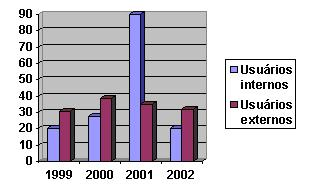
\includegraphics[width=12.5cm,height=7.2cm]{ModeloMonografiaDCCUFRJ-img002.png} 
    \legend{Fonte: Silva, Camargo Pires (2004, p. 45)}
    \label{fig:internet}
\end{figure}


\clearpage
\section{Exemplos de Citações}
{\centering\bfseries\color{red}
Exemplos de Citações
\par}

{\centering\bfseries\color{red}
Citação direta:
\par}

\bigskip

Citações diretas de até 3 linhas, devem iniciar e terminar por aspas duplas.\\

Se o texto original já contiver aspas duplas, substituí-las por aspas simples. A indicação da fonte da citação pode
estar inserida no texto ou após a citação.\\

\bigskip

{\color{red}
Exemplo:}

\bigskip

Segundo Castro (2001, p. 23): {\textquotedbl}Os deveres da conduta do anestesiologista constituem predicados importantes
quando se quer avaliar a qualidade do procedimento.{\textquotedbl}\\

\bigskip

{\color{red}
ou}

\bigskip

{
{\textquotedbl}A expressão 'furiosa' dessa estátua de que fala Rebelais, corresponde também à realidade.{\textquotedbl}
(BAKHTIN, 1987, p. 89).}

\bigskip

{\centering\bfseries\color{red}
Citação Direta com mais de três linhas:
\par}

\bigskip

As citações diretas, no texto, com mais de três linhas, devem ser
destacadas com recuo de 4 cm da margem esquerda, com letra menor que a do texto utilizado e sem as aspas. A indicação da fonte da citação pode estar inserida no texto ou após a citação. \\ 

\bigskip

{\color{red}
Exemplo:}
\bigskip
Sobre mercado financeiro, Fortuna (1996, p. 15) considera:\\
\bigskip

\begin{citacao}
O mercado financeiro permite que um agente econômico qualquer, sem perspectivas de aplicação, em algum empreendimento
próprio, da poupança que é capaz de gerar, seja colocado em contato com outro, cujas perspectivas de investimento
superam as respectivas disponibilidades de poupança.\\
\end{citacao}

\bigskip
A seguir uma citação em inglês:\\

\begin{citacao}[english]
This text is an example in English language in italic with correct hyphenation. This text is an example in English language in italic with correct hyphenation. This text is an example in English language in italic with correct hyphenation.
\end{citacao}
\bigskip

\clearpage{\centering\bfseries\color{red}
Citação Indireta:
\par}

\bigskip

Não se utilizam aspas para esse tipo de citação, nem a(s) página(s) de onde foi extraída a ideia.\\

\bigskip

{\color{red}
Exemplo:}

\bigskip

A bíblia começou a ser escrita no ano 1.000 a.C. e foi finalizada em 100 d.C., com a morte do último apóstolo, São João, levando aproximadamente 1.150 anos para ser concluída \cite{book:GHELLER}.\\


\bigskip

{\centering\bfseries\color{red}
Citação de Citação:
\par}

\bigskip

A indicação da fonte é feita pelo sobrenome do autor da obra citada (não consultada), ano, seguido da expressão latina apud. Após, indica-se o sobrenome do autor da obra consultada, seguido do ano de publicação, precedido por vírgula. Quando for citação direta incluir a(s) página(s) após a data de publicação, precedida de vírgula.\\

\bigskip

{\sffamily
\textrm{\textcolor{red}{Exemplo no texto}}\textrm{:}}

\bigskip

{\sffamily
\textrm{citado por }}

\bigskip

{\sffamily
\textrm{Segundo Marques e Ribeiro}\footnote{\ MARQUES, Alberto; RIBEIRO, \textbf{Angela. As fazendas agrícolas}. São
Paulo: Ática, 2000. 350 p.}\textrm{ (2000 }\textrm{\textcolor{black}{apud }}\textrm{OLIVEIRA, 2001), \apudonline {art:PRADO}{book:AMADO} o Serviço de
Atenção Médico-Sanitário da Suécia tem uma tradição de mais de cem anos. }}

\bigskip

{\color{red}
ou}

{\sffamily
\textrm{\textcolor{red}{Em nota de rodapé}}\textrm{:}}

\bigskip

{\centering\bfseries\color{red}
Indicação da Citação:
\par}

\bigskip

{\sffamily
\textrm{Se a indicação da fonte da citação estiver incluída na frase, a mesma deve aparecer apenas com a inicial
maiúscula seguida de parênteses, com a data de publicação do }\textrm{documento. Quando for citação direta incluir a(s)
página(s) após a data de publicação, precedida de vírgula.}}

\bigskip

{\color{red}
Exemplo com autor pessoal:}

\bigskip

Segundo Fonseca(2004, p. 36): {\textquotedbl}Se não houver mecanismos jurídicos que assegurem a proteção dos direitos
humanos, esse valor não será concretizado pelo Poder Público.{\textquotedbl}\\

\bigskip

{\sffamily
\textrm{\textcolor{red}{Exemplo com dois autores: }}}

\bigskip

Tonetto e Reck (2001, p. 134) destacam: {\textquotedbl}Este autoconhecimento pressupõe conhecer seus limites
[...]{\textquotedbl} \\

\bigskip

{\color{red}
Exemplo com mais de três autores:}

\bigskip

Neste contexto, Couto e outros (2004, p. 52) destacam que: {\textquotedbl}No capitalismo não é a simples ausência do
patrão que promove a superação do despotismo da divisão laboral.{\textquotedbl}\\

\bigskip

{\sffamily
\textrm{\textcolor{red}{Exemplo com autor institucional: }}}

\bigskip

De acordo com a Pontifícia Universidade Católica do Rio Grande do Sul (2001, p. 24): {\textquotedbl}[...] no horizonte 2001/2010, o esforço estratégico da PUCRS será centrado em sete áreas estratégicas [...]{\textquotedbl}\\

\bigskip

{\color{red}
Exemplo sem autor(es), com a entrada pelo título:}

\bigskip

Segundo o Guia de clareamento dental (1996, p. 8): {\textquotedbl}A causa mais comum do escurecimento dental é o tratamento endodôntico realizado de modo inadequado e sem os cuidados técnicos.{\textquotedbl}\\

\bigskip

{\color{red}
Exemplo sem autor(es), com a entrada pelo título que inicia por artigo:}

\bigskip

O movimento social, com o intuito de realizar uma transformação social, é uma das tarefas mais importantes da atualidade
(O COOPERATIVISMO..., 2002).\\

\bigskip

As citações a seguir foram colocadas para que as referências aparecessem na bibliografia. Como exemplo temos os livro de Jorge Amado \cite{book:AMADO}  \cite{book:AMADO2}, e este autor que desconheço \cite{book:OHANSSON}, além de \cite{book:ENGEL} e um artigo \cite{art:PRADO}. Notem que é gerado um link hipertexto no documento em PDF.
